\documentclass[]{../template/Report}%方括号内写yuxi即生成预习报告\documentclass[yuxi]{../template/Report}
\settemplatedir{../template/}%设置模板路径

\exname{示波器的应用} %实验名称
\extable{35} %实验桌号
\instructor{房若宇} %指导教师
\class{信工2401} %班级
\name{姚舜瑜} %姓名
\stuid{3240100532} %学号

\nyear{2025} %年
\nmonth{12} %月
\nday{23} %日
\nweekday{二} %星期几，e.g. \nweekday{三}
\daypart{上午}%上午/下午

\redate{} %如有实验补做，补做日期
\resitu{} %情况说明：

\begin{document}
\maketitle%输出封面

\section{预习报告（10分）}
上课前到学在浙大上完成，注意测试仅1次机会。期末时测试分数会与报告其他部分的分数进行加和处理。

\section{原始数据（20分）}
\begin{figure}[H]
    \centering
    
\includegraphics[width=0.6\textwidth]{figures/实验数据.jpg}
    \caption{自备数据记录草稿纸}
\end{figure}

\section{结果与分析（60分）}
\subsection{数据处理与结果（30分）}
\subsubsection{用比较法验证$f_y = n \cdot f_x$}
\begin{table}[H]
\centering
\caption{比较法测量扫描信号频率}
\label{tab:freq}
\begin{tabular}{|l|l|l|}
\hline
波形个数$n$ & 信号频率$f_y$(\si{\hertz}) & 测得的扫描信号频率$f_x$(\si{\hertz}) \\ \hline
1       & 198.1                & 198.1       \\ \hline
2       & 397.2                & 198.6       \\ \hline
3       & 596.9                & 199.0         \\ \hline
4       & 795.3                & 198.8        \\ \hline
5       & 995.6                & 199.1        \\ \hline
6       & 1194.0               & 199.0        \\ \hline
\end{tabular}
\end{table}
最终结果
\[
\bar{f_x} = \frac{f_1 + f_2 + \cdots + f_5 + f_6}{6} = \frac{198.1+198.6+ 199.0+198.8+199.1+199.0}{6} = \SI{198.43}{\hertz}
\]

扫描时基信号为0.5 \si{\ms \per dit}，即$f_x = \SI{200}{\hertz}$

相对误差
\[
E = \frac{\left|f_\text{实} - f_\text{理}\right|}{f_\text{理}} = \frac{\left| 198.43-200\right|}{200} \times 100\% = 0.785\%
\]


\subsubsection{用李萨如图形测量未知信号的频率}
信号发生器背后输出的~50Hz的电压，作为$f_y$
\begin{table}[H]
\centering
\caption{李萨如图形测量未知信号频率}
\label{tab:li_freq}
\begin{tabular}{|L{0.2\textwidth}|L{0.1\textwidth}|L{0.1\textwidth}|L{0.1\textwidth}|L{0.1\textwidth}|L{0.1\textwidth}|}
\hline
\centering 频率比$f_y:f_x$ & 1:1    & 1:2     & 1:3     & 2:1    & 2:3    \\ \hline
\centering 图形           & \raisebox{-0.5\height}{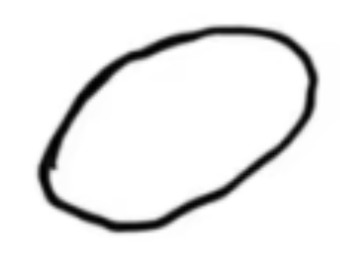
\includegraphics[width=\linewidth]{figures/手绘1.png}} & \raisebox{-0.5\height}{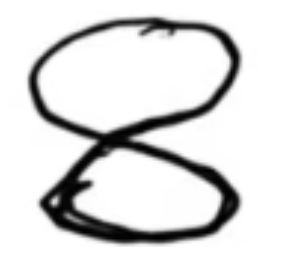
\includegraphics[width=\linewidth]{figures/手绘2.png}} & \raisebox{-0.5\height}{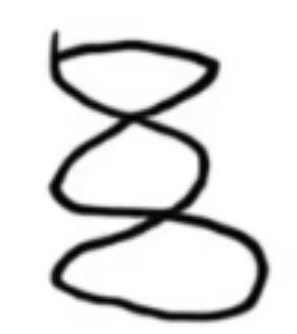
\includegraphics[width=\linewidth]{figures/手绘3.png}} & \raisebox{-0.5\height}{
\includegraphics[width=\linewidth]{figures/手绘4.png}} & \raisebox{-0.5\height}{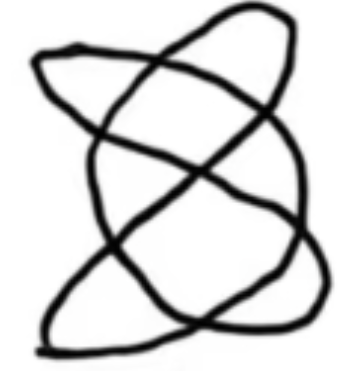
\includegraphics[width=\linewidth]{figures/手绘5.png}} \\ \hline
\centering 垂直交点数$N_y$   & 2      & 4       & 6       & 4      & 6      \\ \hline
\centering 水平交点数$N_x$   & 2      & 2       & 2       & 2      & 4      \\ \hline
\centering 读出$f_x$(\si{\hertz})      & 50.021 & 100.247& 150.178 & 25.006 & 75.026 \\ \hline
\centering 计算$f_y$(\si{\hertz})      & 50.021 & 50.124  & 50.059  & 50.012 & 50.018 \\ \hline
\end{tabular}
\end{table}
平均值
\[
\bar{f_y} = \frac{\sum_{i = 1}^{5}f_{yi}}{5} = \frac{50.021 + 50.124 + 50.059 + 50.012 + 50.018}{5} = \SI{50.047}{\hertz}
\]

相对误差
\[
E = \frac{\left|f_\text{实} - f_\text{理}\right|}{f_\text{理}} = \frac{\left|50.047 - 50\right|}{50} \times 100\% = 0.094\%
\]


\subsubsection{测量二极管正向导通电压}
调整输入信号为正弦波，频率\SI{2}{\kilo\hertz}，幅值约为5$V_{p-p}$，扫描速度为\SI{0.2}{\ms \per div}，用光标法测量结果为：
\begin{table}[H]
\centering
\caption{二极管导通压降}
\label{tab:di}
\begin{tabular}{|L{0.4\textwidth}|C{.2\textwidth}|}
\hline
项目                     & 测量得到的值(\si{\volt }) \\ \hline
输入电压的峰-峰值$U_{1P-P}$    & 4.88               \\ \hline
输出半波电压的峰值$U_{2P}$      & 1.76               \\ \hline
二极管导通的电压降$U_\text{导通}$ & 0.68               \\ \hline
\end{tabular}
\end{table}
其中，二极管导通电压降计算公式为
\[U_\text{导通} = \frac{U_{1P-P}}{2} - U_{2P} = \frac{4.88}{2} - 1.76 = 0.68 \si{\volt}\]

和理论值（硅二极管约为\SI{0.7}{\volt}）相比，相对误差为
\[E = \frac{\left|U_\text{实} - U_\text{理}\right|}{U_\text{理}} = \frac{\left|0.68 - 0.7\right|}{0.7} \times 100\% \approx 2.86\%\]

可以说测量结果与理论值较为接近。
\subsubsection{测量RC电路相位差}
依旧使用上一实验的输入信号，用光标法测量结果为
\begin{table}[H]
\centering
\caption{测量RC电路相位差}
\label{tab:phi}
\begin{tabular}{|C{0.3\textwidth}|C{0.2\textwidth}|C{0.2\textwidth}|}
\hline
\multicolumn{3}{|c|}{实验参数：$R = \SI{750}{\ohm}$，$C = \SI{0.47}{\micro\farad}$,输入信号频率=\SI{2}{\kilo\hertz}} \\
\hline
波形时间差$\Delta T$(\si{\milli\second}) & 周期$T$(\si{\milli\second}) & 相位差$\Delta \varphi$ \\ \hline
0.104                     & 0.504         & $74^\circ 17' 24''$            \\ \hline
\end{tabular}
\end{table}
其中，相位差计算公式为
\[\Delta \varphi = \frac{\Delta T}{T} \times 360^\circ = \frac{0.104}{0.504} \times 360^\circ \approx 74.29^\circ = 74^\circ 17' 24''\]

\textbf{理论值验证：}
根据测量周期 $T = \SI{0.504}{\ms}$，可得信号频率 $f = 1/T \approx \SI{1984.1}{\hertz}$，角频率 $\omega = 2\pi f \approx \SI{12466.6}{\radian\per\second}$。
RC串联电路（测量电容电压）的理论相位差为：
\[ \varphi_{\text{理}} = \arctan(\omega RC) = \arctan(12466.6 \times 750 \times 0.47 \times 10^{-6}) \approx \arctan(4.3945) \approx 77.18^\circ = 77^\circ 10' 48'' \]

相对误差：
\[ E = \frac{|\varphi_{\text{实}} - \varphi_{\text{理}}|}{\varphi_{\text{理}}} = \frac{|74.29 - 77.18|}{77.18} \times 100\% \approx 3.7\% \]

可以说测量值与理论值也是相当接近。
\subsection{误差分析（20分）}
从整体数据来看，本次实验的测量精度较高，各项目的相对误差均控制在较小范围内。但在实验过程中，仍存在以下几类不可忽视的误差来源：

\begin{enumerate}
    \item \textbf{读数与视觉误差（随机误差）}
    \begin{itemize}
        \item \textbf{示波器线宽度影响：} 示波器屏幕上显示的波形线条并非理想的几何细线，而是具有一定的宽度。在使用光标法测量电压峰峰值或时间间隔时，光标线与波形边缘的对齐存在主观判断偏差。
    \end{itemize}

    \item \textbf{仪器本身的系统误差}
    \begin{itemize}
        \item \textbf{信号源的偏差与漂移：} 信号发生器的显示频率与实际输出频率可能存在微小偏差。例如在验证 $f_y = n \cdot f_x$ 时，理论扫描频率应为 \SI{200}{\hertz}，但实测平均值为 \SI{198.43}{\hertz}，这表明信号源输出或示波器时基本身存在约 \SI{0.785}{\percent} 的系统偏差。此外，信号源长时间工作后可能产生温漂，导致频率微小波动。
    \end{itemize}

    \item \textbf{实验元件的标称误差}
    \begin{itemize}
        \item 在测量RC电路相位差时，理论值的计算依赖于电阻 $R$ 和电容 $C$ 的标称值（\SI{750}{\ohm} 和 \SI{0.47}{\micro\farad}）。实际上，电子元器件通常有 $5\% \sim 10\%$ 的容差，实际值与标称值的差异是导致该项目产生 \SI{3.7}{\percent} 相对误差的重要原因之一。
    \end{itemize}
\end{enumerate}

综上所述，通过多次测量取平均值有效降低了随机误差的影响，但仪器和元件的固有偏差是系统误差的主要来源。

\subsection{实验探讨（10分）}

本次实验让我成功地掌握了示波器的基本使用方法及其在电子测量中的重要应用。通过比较法和李萨如图形法测量频率，我深刻理解了示波器如何将时间域信号转换为空间域波形显示的原理。此外，测量二极管导通电压和RC电路相位差的实验环节，使我体会到示波器在实际电子元件特性分析中的实用价值。
在动手实验过程中，我也掌握了一些实操小技巧，如调整波形上下一样大、使用触发功能稳定波形显示等，这些都让我对示波器更加了解并数量运用。
\section{思考题（10分）}

\subsection{示波器为什么能显示被测信号的波形}
电子先是通过加速电场进入轴线。
\subsubsection{垂直偏转（Y 轴）}
\begin{itemize}
    \item \textbf{信号输入：} 待测信号电压 $u(t)$ 被加载至 Y 轴偏转板，即 $u_Y = u(t)$。
    \item \textbf{偏转机制：} 电子束穿过偏转板时受电场力作用发生偏转，最终轰击荧光屏。垂直位移 $y$ 与偏转电压 $u_Y$ 呈线性关系：
    \[ y = \frac{L l_y}{2 d_y U_a} u_Y \]
    式中 $L$ 为偏转板中心至屏幕距离，$l_y, d_y$ 为偏转板尺寸参数，$U_a$ 为加速电压。
    \item \textbf{结论：} 对于特定示波器，系数为常数，故 $y \propto u(t)$。
\end{itemize}

\subsubsection{水平偏转（X 轴）}

电子束同时也会经过 X 轴偏转极板。

\begin{itemize}
    \item \textbf{扫描电压：} X 轴施加周期性线性变化的锯齿波电压 $u_X(t)$。在扫描周期 $T_x$ 内，电压随时间均匀增加：$u_X(t) = k t$。
    \item \textbf{水平位移：} 类似地，水平位移 $x$ 正比于 $u_X$：
    \[ x = \frac{L l_x}{2 d_x U_a} u_X \]
    \item \textbf{结论：} 结合扫描电压特性，实现了 $x \propto t$。
\end{itemize}

\begin{figure}[H]
    \centering
    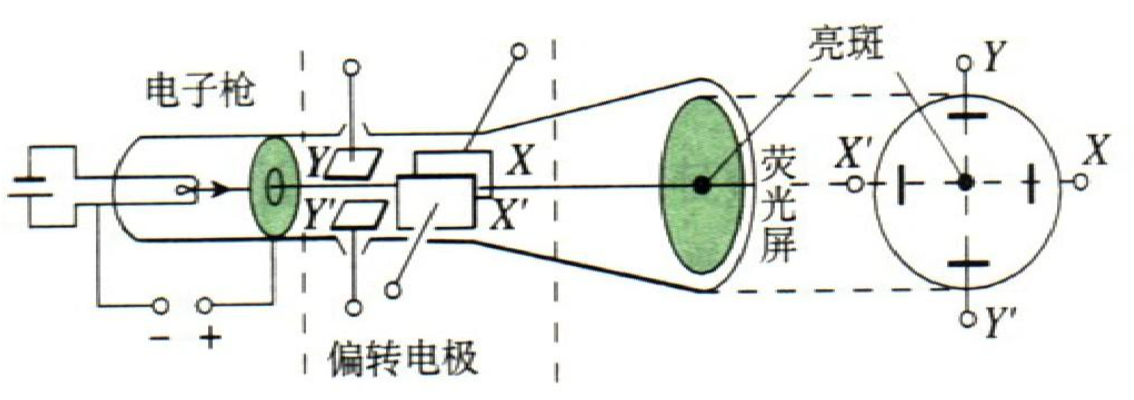
\includegraphics[width=0.5\textwidth]{figures/示波器原理.png}
    \caption{示波器显示原理}
\end{figure}

示波器利用锯齿波扫描，将信号的时间函数 $(t, u(t))$ 转化为屏幕平面的几何坐标 $(x, y)$：
\begin{itemize}
    \item $x(t) \propto t$ （时间轴）
    \item $y(t) \propto u(t)$ （信号幅度）
\end{itemize}
这样，电子束在屏幕上扫过的轨迹 $y(x)$，就精确地复现了被测信号 $u(t)$ 的波形。

当扫描电压的周期 $T_x$ 恰好是信号周期 $T_y$ 的整数倍（即 $T_x = nT_y$）时，后续扫描的波形会与前一次的轨迹完全重合，我们就能观察到清晰、稳定的波形。

但如果其中有相位差，那么波形可能会左右移动。
\subsection{在观察李萨如图形时为什么总是不断地来回翻转，反转快慢受哪些因素影响}
\paragraph{翻转的原因}两个信号的频率并不是严格的整数比，可能有一定的相位差，所以不能形成稳定的李萨如图形，导致李萨如图形不停翻转变化。
\paragraph{翻转快慢的因素}翻转快慢就是相位差改变的快慢，这与两个信号频率的整数倍之间的差值$\left|pf_x - qf_y\right|$有关（其中$p,q$互质）

\subsection{切实理解示波器同步的概念，如果发生波形左移或右移应该如何调整才能使其稳定下来}
\paragraph{同步}被测信号的频率如果是扫描信号整数倍时，每次都能保证波形最左端为相同相位，即示波器所显示波形不会移动，如果两者之间有一定相位差，则被扫描到的相位将会不断变化，导致波形左移或右移。
\paragraph{调整}使用\textrm{TRIG LEVEL} 按钮调整触发电平高低，使得每次抓取到的信号都保持在同一相位，就可以使波形稳定下来，不会左右移动。
\insertnotes
\end{document}